\chapter{序論}
\thispagestyle{empty}
\label{chap1}
\graphicspath{{chap1/figure/}}
\minitoc

%%%%%%%%%%%%%%%%%%%%%%%%%%%%%%%%%%%%%%%%%%%%%%%%%%%%%%%%%%%%%%%%%%%%%%%%%%%%


% ================================================== %
% section
% ================================================== %
\newpage
\section{研究の意義・背景}
\label{chap1_background}

通常、我々が天体を観測するとき、可視光を通してその形状や特徴を観察する。
一方で、天文学では熱や電磁波、放射線といった可視光以外の媒体を通じて様々な現象が明らかにされてきた。
中でも、電磁波の一種であるx線を観測することは、天文学において非常に有用である。
2018年に打ち上げられたFOXSI3では太陽コロナのx線写真を撮影することに成功し、その物理をより明らかにするに至った。
図\ref{fig:foxsi-fullsun-image}はその撮影像の1枚である。
太陽コロナを満たす高温のプラズマから放射される電磁波はX線の領域であり、これを撮影することは長年の課題であった。
X線は大気により吸収されやすいという特徴を持つため、宇宙に打ち上げられたロケットから観察する必要があるためである。
さらに、時間分解能と空間分解能の両方を十分に確保して撮影しなければならず、非常に難しい問題であった。
これを可能にした一つの要素として、Wolter型ミラーが挙げられる。

\begin{figure}[h]
\centering
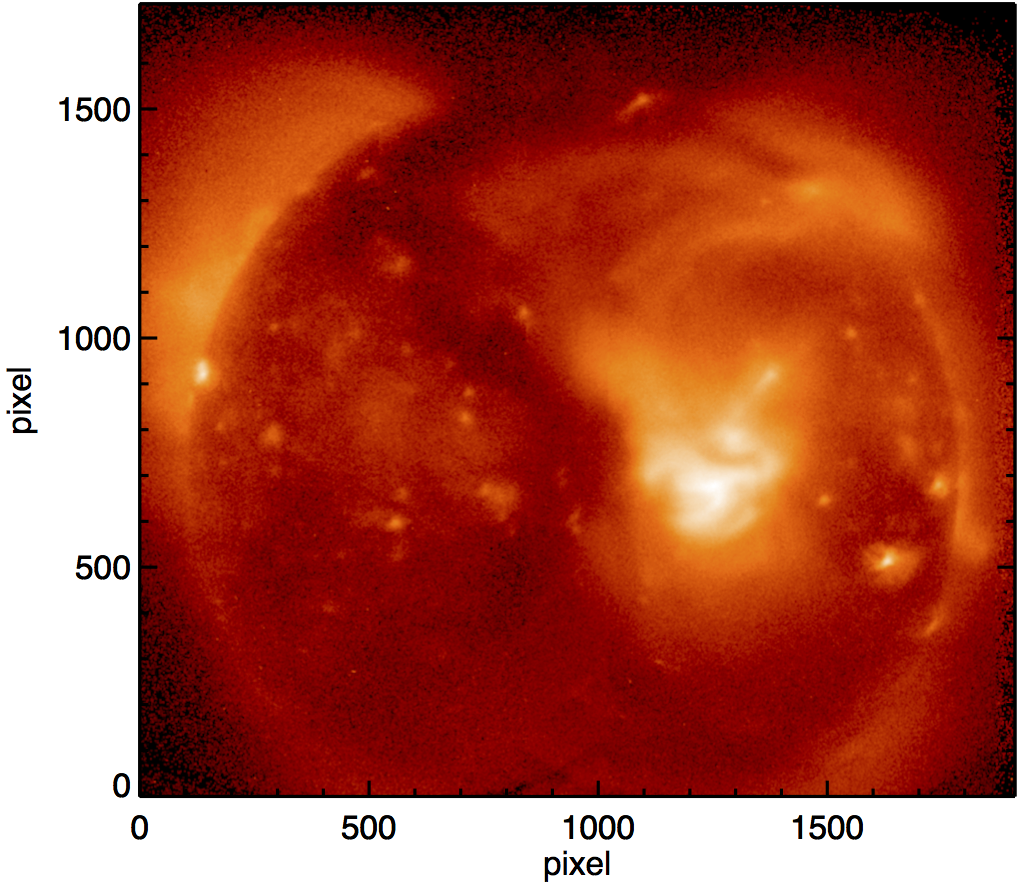
\includegraphics[width=8cm]{foxsi3-full-sun.png}
\caption{FOXSI-3 phoenix full sun soft X-ray image}
\label{fig:foxsi-fullsun-image}
\end{figure}

\clearpage
% -------------------------------------------------- %
% section
% -------------------------------------------------- %
\newpage

\section{Wolterミラー}
\label{chap1_wolter_mirror}

\begin{figure}[b]
\centering
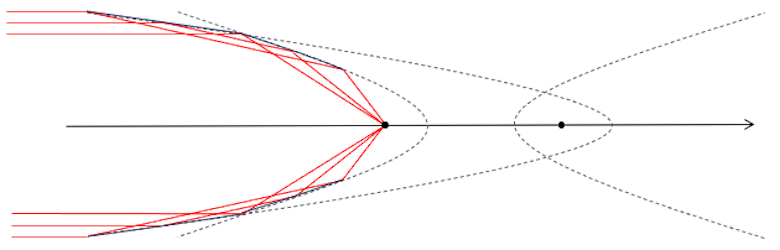
\includegraphics[width=10cm]{wolter_type_1.png}
\caption{Wolter I型}
\label{fig:wolter_type_1}
\end{figure}

\begin{figure}[b]
\centering
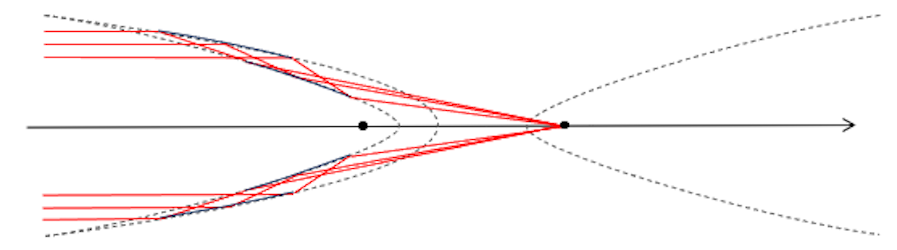
\includegraphics[width=10cm]{wolter_type_2.png}
\caption{Wolter II型}
\label{fig:wolter_type_2}
\end{figure}

\begin{figure}[b]
\centering
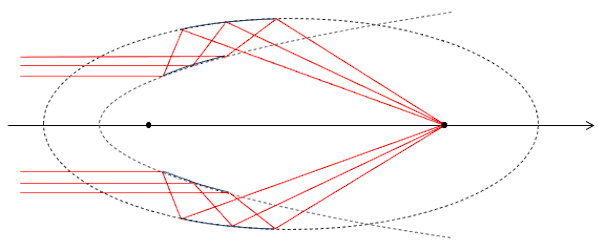
\includegraphics[width=10cm]{wolter_type_3.png}
\caption{Wolter III型}
\label{fig:wolter_type_3}
\end{figure}

光を一点に集光するための素子として、屈折を利用するレンズ、反射を利用したミラー、回折を利用したフレネルゾーンプレートなどが有名である。

WolterミラーにはI型(図\ref{fig:wolter_type_1})、II型(図\ref{fig:wolter_type_2})、III型(図\ref{fig:wolter_type_3})の3種類が存在し、それぞれに長所と短所が存在する。
I型は放物面、双曲面の順にいずれも内面において反射する構成になっており、後述するマンドレル転写加工がしやすいため高精度な作製が期待できる。
II型は放物面内面、双曲面外面の順に反射する構成になっている。I型に比べ加工・設置が難しくなるが、内面と外面を重ねた配置にすることができ、焦点距離を短くし光学系全体を小型化することができる。
III型のX線への応用は未だに進んでいない。

\clearpage
% -------------------------------------------------- %
% section
% -------------------------------------------------- %
\newpage

\section{本研究で測定対象となるWolterミラーの設計}
本研究において測定対象となるのは、FOXSI-4での利用が検討されている天体望遠鏡用のWolterミラーであり、放物面、双曲面の順に反射するI型に分類される。
現在、回転体ミラーの加工では凸形状のマンドレルを高精度に加工し、そこに金属材料を転写するという方式が非常に有利であり、反射面がいずれも内側になるWolter I型が採用されている。
また、放物面と双曲面が連続に接続されている方が端面が存在しないぶん加工精度の点で有利であるため、そのような構成となっている。
以下では、開発対象となっているWolter I型のミラーの設計パラメータを図\ref{fig:wolter_params}に対応して表\ref{tb:wolter_params}に示す。

\begin{figure}[h!]
\centering
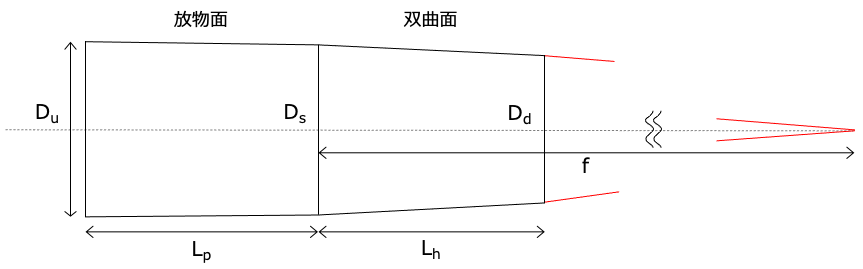
\includegraphics[width=12cm]{wolter_mirror_params.png}
\caption{Wolterミラーの設計変数}
\label{fig:wolter_params}
\end{figure}

\begin{table}[ht]
\begin{center}
  \begin{tabular}{|c|c|l|} \hline
    変数 & 値 & 説明 \\ \hline
    $d_u$ & 60.801 mm & 上流端開口直径 \\
    $d_s$ & 60.000 mm & 接合部直径 \\
    $d_d$ & 57.689 mm & 下流端開口直径 \\
    $l_p$ & 102.501 mm & 放物面部長さ \\
    $l_h$ & 97.499 mm & 双曲面部長さ \\
    $ml$ & 200.000 mm & ミラー全長 \\
    $f$ & 2000.000 mm & 焦点距離 \\ \hline
  \end{tabular}
  \caption{Wolterミラー各設計変数の値}
  \label{tb:wolter_params}
\end{center}
\end{table}

これらを図\ref{fig:wolter_profile}のように放物面部および双曲面部の設計半径として表すと、下式(パラメータは図\ref{tb:wolter_profile_constants})のようになる。
$f1$は座標系の平行移動に関して任意であるため、変数として表記する。

\begin{equation}
    r_p(z) = \sqrt{ -4p(z - p - f_2) } \\
\end{equation}

\begin{equation}
    r_h(z) = b \sqrt{ \frac{(z - (f_1 + f2) / 2)^2}{a^2} - 1.0 }
\end{equation}

\begin{figure}[h]
\centering
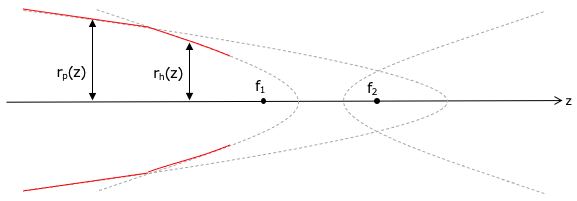
\includegraphics[width=10cm]{mirror_profile.png}
\caption{Wolterミラーの設計半径}
\label{fig:wolter_profile}
\end{figure}

\begin{table}[htb]
    \begin{center}
      \begin{tabular}{|c|c|l|} \hline
        定数 & 値 & 説明 \\ \hline
        $p$ & 0.0562 mm & 下流端開口直径 \\
        $a$ & 1000.056 mm & 放物面部長さ \\
        $b$ & 10.606 mm & 双曲面部長さ \\ 
        $f_1$ & 任意 & 焦点座標 \\
        $f_2$ & $f_1 + \sqrt{ a^2 + b^2 }$  & 共焦点座標 (双曲線のもう一方の焦点) \\\hline
      \end{tabular}
      \caption{Wolterミラーの設計半径における定数}
      \label{tb:wolter_profile_constants}
    \end{center}
\end{table}

\clearpage
% -------------------------------------------------- %
% section
% -------------------------------------------------- %
\newpage
\section{本論文の目的}
\label{chap1_purpose}


\clearpage
% -------------------------------------------------- %
% section
% -------------------------------------------------- %
\newpage

\section{本論文の構成}
\label{chap1_outline_of_paper}


%%%%%%%%%%%%%%%%%%%%%%%%%%%%%%%%%%%%%%%%%%%%%%%%%%%%%%%%%%%%%%%%%%%%%%%%%%%%%
%%% Local Variables:
%%% mode: katex
%%% TeX-master: "../thesis"
%%% End:
